\documentclass[11pt]{article}
\usepackage[margin=1in]{geometry}
\usepackage{graphicx}
\usepackage{booktabs}
\setlength{\emergencystretch}{3em}
\usepackage{longtable}
\usepackage{amsmath,amssymb}
\usepackage{multirow}
\usepackage{natbib}
\usepackage{xcolor}
\usepackage{microtype}
\usepackage{caption}
\usepackage{subcaption}
\usepackage[hidelinks]{hyperref}
\title{Batch-transductive prediction of WXS mutation burden across TCGA and CPTAC}
\author{}
\date{}
\begin{document}
\maketitle

\begin{abstract}
Tumor mutational burden (TMB) is used as background context for immunotherapy, while this study predicts an operational WXS-derived non-synonymous mutation burden (WMB). Because our label is a unique variant count without callable-territory normalization, WMB should not be read as a clinical TMB measurement; sequencing assay and cohort differences make transcriptomic surrogates difficult to transport. We evaluated a batch-transductive, two-way external prediction problem in which expression profiles from one cohort are used to predict mutation burden in a second cohort after an unlabeled adaptation batch is observed. The study combines 2,431 TCGA and 1,646 CPTAC-3 cases with open whole-exome mutation calls and matched RNA expression. Labels were reconstructed by coordinate-and-allele deduplication of an explicitly defined non-synonymous variant set and transformed as log1p counts before any split. We compare source-mean, ridge, elastic-net, PCA-histogram gradient boosting, and a neural baseline with an assay-aware heteroscedastic regressor. The latter learns a shared expression representation, a mean and variance head, and a gradient-reversal cohort discriminator using only source labels and unlabeled target adaptation expression. Across three fixed seeds, the confirmatory refit compares the candidate with baselines trained under the same source-label access on a disjoint target evaluation subset. Prediction intervals are reported as source-calibrated and are stress-tested for target undercoverage; attribution and lineage analyses are treated as conditional audits rather than biological validation.
\end{abstract}

\section{Introduction}
Tumor mutational burden is the number of somatic mutations carried by a tumor, usually normalized to a callable genomic territory. It is a compact summary of genomic instability and mutational processes, and it has been associated with response to immune checkpoint blockade across cancer types \citep{ZR2017f004a,RM2019bd13b,AM2017f218c,DL2021e47f7}. The biomarker is clinically attractive because it can separate tumors with a large neoantigen opportunity from tumors with fewer coding alterations, yet its interpretation depends on the sequencing panel, filtering rules, tumor purity, and the definition of an eligible variant \citep{M2017ddb97,MD2018d4430,D20209d1b5}. The same tumor can consequently receive different numerical TMB values in different assays. Our WMB target intentionally retains this assay dependence as an operational non-synonymous count rather than claiming clinical normalization. This assay sensitivity creates a practical problem for computational biomarker development: a model that predicts WMB within one study can appear accurate while learning study-specific signals that do not transport.

RNA expression offers a complementary view of the processes that generate and expose mutation burden. Replication stress, DNA repair deficiency, immune activation, lineage state, and tumor purity all leave transcriptional signatures. RNA-based estimation is appealing when matched normal DNA or broad exome sequencing is unavailable, and recent work has shown that mutational burden can be estimated from RNA sequencing with careful modeling of sequencing context \citep{Bailey2022TMBRNA}. Other efforts have inferred WMB from histopathology or multimodal inputs \citep{Huang2022TMBHistology}. These studies establish feasibility but do not answer a stricter transport question: can a model trained in one large study predict a corrected WMB definition in a second study collected with another protocol, and can it report uncertainty when the transport is poor?

The Cancer Genome Atlas (TCGA) and Clinical Proteomic Tumor Analysis Consortium (CPTAC) provide a useful test because both contain molecularly characterized tumors while differing in sample processing, sequencing pipelines, cohort composition, and lineage balance \citep{CancerGenomeAtlas2013,Mertins2016CPTAC,DJ201966234}. We formulate two external directions, TCGA to CPTAC and CPTAC to TCGA, rather than pooling the cohorts and randomly splitting patients. Each target cohort is divided into an unlabeled adaptation subset and a disjoint labeled evaluation subset before model fitting; target labels are consumed only for the final score. The setting is therefore batch-transductive and does not claim inductive single-patient deployment.

We make four contributions. First, we define and audit a deduplicated WXS-based target that avoids counting the same variant multiple times across files while preserving the biological distinction between high and low burden. Second, we evaluate an assay-aware heteroscedastic predictor that combines a shared expression encoder, a supervised Gaussian likelihood, and an unlabeled target-domain discriminator; these are established components rather than a new algorithm. Third, we use a fixed source-only development and all-source refit protocol, with a disjoint target adaptation/evaluation split, four primary metrics, matched ablations, perturbation tests, lineage-stratified error, and interval coverage. Fourth, we use gradient-times-input attributions to audit model reliance in each direction while testing attribution instability. We do not claim that the architecture is the first domain adaptation method, that the endpoint is clinical TMB, or that any gene is a universal WMB marker.

\section{Related work and problem positioning}
\subsection{WMB as a context-dependent genomic measurement}
Large-scale surveys established that mutation burden varies widely across tumor lineages and is shaped by age, environmental exposure, DNA repair, and mutational processes \citep{ZR2017f004a,RM2019bd13b}. Clinical studies connected high burden to checkpoint blockade response in selected settings, including melanoma, lung cancer, and pan-tumor cohorts \citep{MD2018d4430,AM2017f218c,PA2019f4932}. Methodological studies showed that panel size, callable territory, filtering, and variant class change the numerical value of WMB \citep{M2017ddb97,D20209d1b5}. WMB is therefore a biological signal observed through an assay, rather than a perfectly invariant patient attribute. Our target follows this view: it is a frozen, explicitly defined WXS-derived count, and the prediction task is to transport that definition across cohorts.

\subsection{Expression and multimodal surrogates}
Expression-based surrogates exploit the fact that genomic instability, immune interaction, and lineage state alter transcriptional programs. RNA-sequencing estimation without a matched normal sample demonstrated that tumor transcriptomes contain information about mutation burden, but also emphasized sequencing context and depth \citep{Bailey2022TMBRNA}. Histopathology and clinical multimodal models provide a complementary precedent for TMB estimation \citep{Huang2022TMBHistology}; radiomic and histopathologic models similarly report useful within-cohort discrimination. These approaches differ from the present problem in two ways. They commonly use one cancer type or one data source, and they often optimize one discrimination or correlation statistic. We instead evaluate a continuous WXS-count target, require agreement across four primary metrics, and separate unlabeled target adaptation from labeled external scoring.

\subsection{Cohort-scale molecular resources}
TCGA made matched genomic and transcriptomic profiles available at pan-cancer scale and enabled systematic studies of tumor lineages and molecular subtypes \citep{CancerGenomeAtlas2013}. CPTAC adds quantitative proteomics and an independent sample-processing context, with proteogenomic studies showing how somatic events propagate through signaling networks \citep{Mertins2016CPTAC,DJ201966234}. The two resources are complementary but not exchangeable: their patient composition, extraction protocols, sequencing centers, and processing pipelines differ. A model that performs on a pooled random split can exploit shared technical structure and yield over-optimistic estimates. The two-way design used here turns this resource difference into an explicit stress test.

\subsection{Domain adaptation, uncertainty, and interpretation}
Domain-adversarial training was introduced to learn representations that are predictive while reducing domain discriminability \citep{Ganin2016DANN}. Alignment can remove technical effects but may also remove biological variation that is predictive in one direction and absent in another, so we treat it as a hypothesis to test by ablation. Heteroscedastic likelihoods model input-dependent noise, while Bayesian and ensemble approaches separate epistemic from observation uncertainty \citep{Kendall2018Uncertainty}. Our variance head provides a patient-level scale that can be calibrated on source residuals and audited on target patients; it does not claim fully Bayesian uncertainty. Integrated gradients and SHAP provide complementary attribution frameworks \citep{Sundararajan2017IG,Lundberg2017SHAP}, but correlated genes and cohort composition can make rankings unstable. We therefore use attributions as an explicit stability analysis rather than as causal evidence.

\subsection{What this study tests}
The contribution is an evidence-bounded evaluation of a complete prediction system. The model, splits, primary metrics, and three seeds are defined before external target labels are consumed. The baseline suite spans constant, linear, tree, and neural predictors. Additional analyses test whether the result depends on a mechanism, a clean expression matrix, a pooled average, a point estimate, or a particular interpretation. This design distinguishes a model that transports one target definition from a benchmark that only ranks methods within one cohort.

The broader biomarker literature also motivates each control. Pan-cancer sequencing studies describe mutational landscapes and their clinical associations \citep{A20181e9e4,PM202299bdd,Y202033ae9,TA2019c6103,R20183350e,BC20191812e,PS20205cb68,PM20181fbc2}. Checkpoint studies connect burden to treatment response but emphasize tumor type, assay, and treatment context \citep{F2021d1922,RS2020b4e8b,C20200d165,A2022816e6,G202190cac,YH202072c0b,H2018a0678,X20209c79a,AC2019b5978}. Reviews and clinical series document threshold sensitivity, blood-versus-tissue differences, and uncertainty in translating WMB across platforms \citep{LR2023dd859,J2018b4421,PY2020d45d6,H2019557b0,DL2021e47f7,AM201808061,EB201917903,PT2016dead7}. Transcriptomic and immune-state studies provide plausible biological links between expression and genomic instability \citep{DR201894b95,S2019d1269,F20241e1be,MD201820035,D20190effa,AL2020b5a9f,J2021c7974,A2023f2564}. Finally, pan-cancer molecular atlases, proteogenomic studies, and expression-based signatures motivate external cohort validation rather than random splitting \citep{CM20212afeb,K20219ece3,A20208c510,F20199dd64,SL20205ea48,R20195cc8a,AJ202033d96,WL202355f55}.

\section{Results}
\subsection{A corrected cross-cohort target and two-way evaluation}
We obtained neutral GDC STAR-count expression files and open masked WXS mutation files for cases with exact GDC case identifiers. For each case, all qualifying non-synonymous variants were merged across available WXS files and deduplicated by chromosome, start, end, reference allele, and alternate allele. The resulting unique non-synonymous count was transformed as $y=\log(1+\mathrm{WXSCount})$. No expression measurement entered label construction. After requiring both expression and a usable WXS label, 4,077 patients remained: 2,431 TCGA and 1,646 CPTAC-3. The expression matrix contains 4,096 genes selected before model fitting and is standardized using source training patients only. Cohort identity is retained as metadata and is never used as a target label.

The primary design has six external evaluations: two source--target directions and seeds 11, 23, and 47. In TCGA$\rightarrow$CPTAC, each model sees 1,944 TCGA training patients and 487 source-validation patients during model development; the CPTAC cohort is divided into an unlabeled adaptation subset and a disjoint external evaluation subset. In CPTAC$\rightarrow$TCGA, the corresponding source split contains 1,316 training and 330 validation patients, and the TCGA cohort is divided in the same way. The source validation set is used only to estimate the residual scale factor for predicted standard deviations; the 50-epoch schedule is fixed and no external checkpoint is selected. Only adaptation expression, without labels, is visible to the domain discriminator; evaluation patients are absent from training. Target labels are loaded as metadata but are consumed only for the final external score. This is a batch-transductive protocol in which an unlabeled adaptation batch is available before prediction, rather than an inductive single-patient protocol.

The two target distributions are not interchangeable. The median transformed burden is approximately 4.1 in both cohorts, but the upper tail extends above 9 in each direction and the lineage mixture differs. TCGA contributes eight recurrent labels in this analysis (GBM, KIRC, LAML, LUAD, PAAD, SKCM, STAD, and UCEC), and CPTAC has a different count for each label. After averaging repeated seed predictions for descriptive summaries, unique held-out patient counts per lineage range from 124 to 300 for TCGA$\rightarrow$CPTAC and from 93 to 453 for CPTAC$\rightarrow$TCGA. This imbalance is a reason to report patient counts and stratified error rather than treating every lineage as equally precise.

We performed three label and identity checks before model fitting. First, exact case identifiers were required for both expression and WXS files; partial string matches were rejected. Second, variant counts were compared before and after coordinate-and-allele deduplication, and cases with no qualifying variants were retained as zero-count cases rather than silently removed. Third, a forward audit confirmed that the label-building routine never loads expression values and that source-derived standardization is computed separately for each seed. These checks address a common leakage route in which a transcriptomic matrix is accidentally used to filter or define its own target.

\begin{figure}[t]
\centering
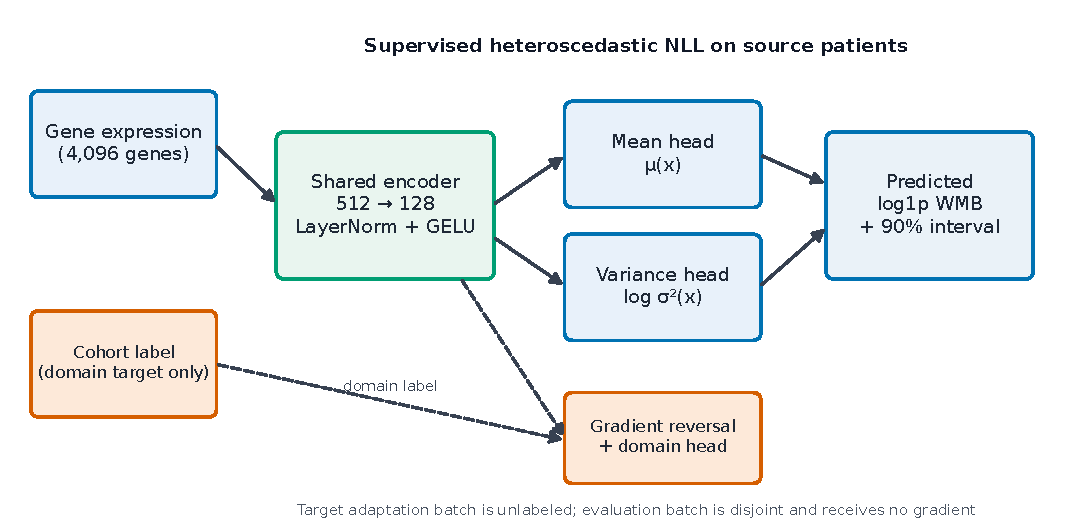
\includegraphics[width=\linewidth]{../results/figures/figure1_mechanism.pdf}
\caption{Assay-aware heteroscedastic model and batch-transductive split. Source expression and the unlabeled target adaptation half pass through a shared encoder. The source patients optimize a heteroscedastic Gaussian likelihood for mean $\mu(x)$ and log variance $\log\sigma^2(x)$; the adaptation half contributes only to the gradient-reversal domain head. The disjoint target evaluation half receives no training gradient and is used only for final scoring. The output is a log1p WMB estimate and a source-calibrated 90\% interval.}
\label{fig:mechanism}
\end{figure}

\subsection{Assay-aware prediction in the confirmatory external comparison}
The model mechanism is shown in Fig.~\ref{fig:mechanism}. The encoder is a 4,096-to-512 linear projection with layer normalization, GELU activation and dropout, followed by a 512-to-128 projection. The mean head predicts the conditional center and the variance head predicts log variance. The source loss is
\begin{equation}
\mathcal{L}_{\mathrm{NLL}}=\frac{1}{2}\left[\exp(-\ell)(y-\mu)^2+\ell\right],\qquad \ell=\mathrm{clip}(\log\sigma^2,-6,4),
\end{equation}
while a gradient-reversal discriminator receives source and target representations. Its binary cross-entropy term is added with an annealed coefficient that reaches 0.35. The architecture, optimizer, and fixed 50-epoch budget were frozen from source-only development. The final candidate was then refit on all source patients before target labels were consumed for scoring, matching the source-data usage of the conventional baselines. The domain discriminator received only the unlabeled adaptation subset; the held-out evaluation subset was absent from representation alignment.

Figure~\ref{fig:main} summarizes the six confirmatory held-out runs. In TCGA$\rightarrow$CPTAC, the assay-aware refit achieved RMSE $0.888\pm0.024$, MAE $0.642\pm0.026$, Spearman $0.775\pm0.012$, and $R^2=0.662\pm0.015$ over seeds. In the reverse direction, values were RMSE $1.030\pm0.029$, MAE $0.754\pm0.033$, Spearman $0.729\pm0.019$, and $R^2=0.554\pm0.030$. On the identical held-out target cases, PCA-histogram boosting reached RMSE $1.032\pm0.034$ and $R^2=0.544\pm0.011$ in the first direction and RMSE $1.180\pm0.035$ and $R^2=0.416\pm0.031$ in the second. The candidate improved all four primary metrics in every seed and direction relative to PCA-HGB. Against the adaptation-aware CORAL-PCA-HGB control, the candidate retained lower mean RMSE and higher mean Spearman correlation and $R^2$ in both directions; reverse-direction MAE was nearly tied (0.754 versus 0.756), with mixed per-seed differences. The comparison is batch-transductive: the candidate receives unlabeled adaptation expression, whereas PCA-HGB and the mean-only MLP are inductive controls. The heteroscedastic no-domain ablation is an additional inductive neural control, while the homoscedastic-domain ablation is an equally transductive alignment control. We therefore interpret the candidate gain as conditional on access to an unlabeled target batch rather than as a universal advantage.

\begin{figure}[t]
\centering
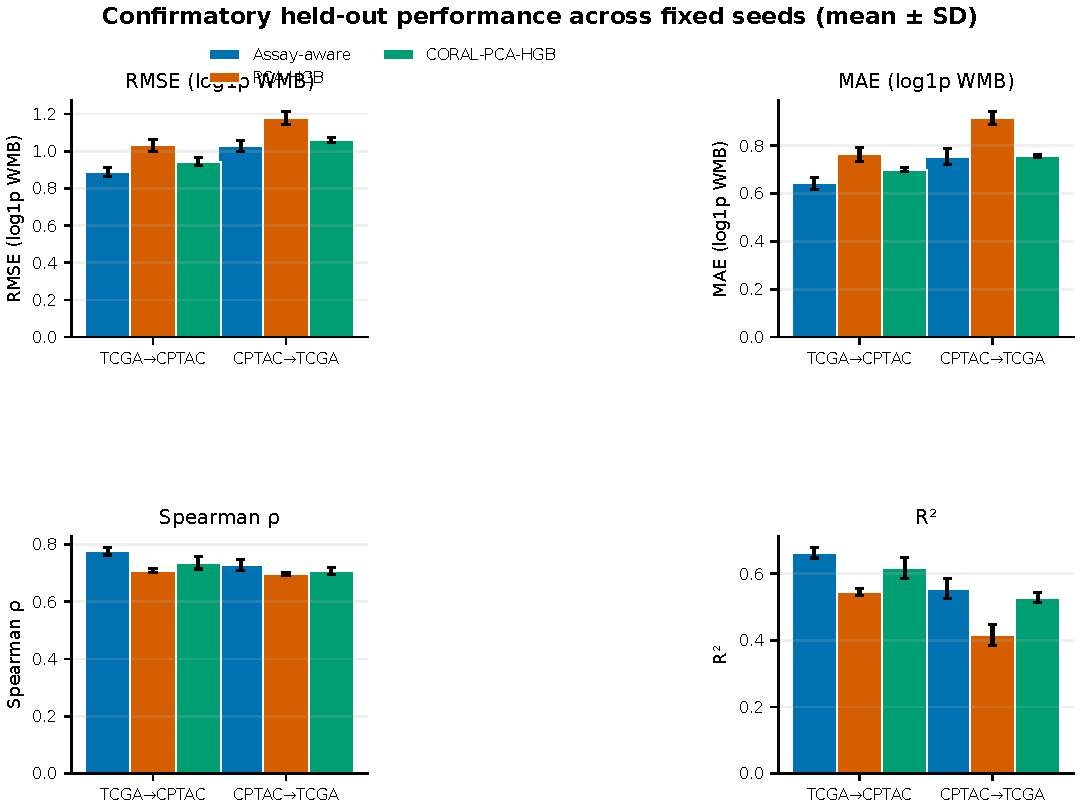
\includegraphics[width=\linewidth]{../results/figures/figure2_main.pdf}
\caption{Confirmatory held-out performance over three fixed random seeds. Bars show mean and standard deviation for the assay-aware refit, PCA-histogram boosting, and adaptation-aware CORAL-PCA-HGB on identical target evaluation cases in each direction (823 CPTAC cases per seed and 1,216 TCGA cases per seed); black points show the individual seed values. Insets show paired candidate-minus-CORAL differences with 95\% patient-bootstrap intervals (2,000 resamples per seed), with rows ordered TCGA$\rightarrow$CPTAC then CPTAC$\rightarrow$TCGA; negative values favor the candidate for RMSE/MAE and positive values favor it for Spearman correlation/$R^2$.}
\label{fig:main}
\end{figure}

The paired comparison against PCA-histogram boosting is consistent at the seed level. For TCGA$\rightarrow$CPTAC, RMSE improvements were 0.144, 0.124, and 0.162 log1p units for seeds 11, 23, and 47; Spearman gains were 0.063, 0.056, and 0.081. For CPTAC$\rightarrow$TCGA, RMSE improvements were 0.114, 0.167, and 0.168 and Spearman gains were 0.017, 0.033, and 0.047. Every paired seed improved in all four primary metrics on the same held-out cases. Patient-level bootstrap intervals for the candidate-minus-CORAL comparison are reported as descriptive uncertainty and are not used to select the architecture.

Table~\ref{tab:baseline} gives the compact mean-over-seeds external comparison for matched held-out cases. The source-mean control had negative $R^2$ in both directions and is omitted from the compact table. Ridge and elastic-net fit the source expression strongly but lose transport performance, illustrating that high validation accuracy is insufficient when the cohort changes. PCA-histogram boosting is the strongest inductive baseline. We also include a CORAL-PCA-HGB control that uses the same unlabeled adaptation batch as the candidate to align source and target covariance before boosting. The assay-aware model improves most on the reverse direction, where the conventional model has a larger error and positive bias. The confirmatory mean-only MLP is an inductive capacity control: adding a nonlinear encoder without target adaptation does not recover the gain. The homoscedastic-domain control provides a transductive alignment comparison with the same target-batch access but no input-dependent variance head.

\begin{table}[t]
\centering
\caption{Mean confirmatory external metrics across three seeds on identical held-out target cases. RMSE and MAE are lower-is-better; Spearman correlation and $R^2$ are higher-is-better.}
\label{tab:baseline}
\begin{tabular}{llrrrr}
\toprule
Direction & Model & RMSE & MAE & Spearman & $R^2$\\
\midrule
TCGA$\rightarrow$CPTAC & Ridge & 1.262 & 0.964 & 0.609 & 0.319\\
TCGA$\rightarrow$CPTAC & Elastic-net & 1.187 & 0.873 & 0.666 & 0.398\\
TCGA$\rightarrow$CPTAC & PCA-HGB & 1.032 & 0.763 & 0.709 & 0.544\\
TCGA$\rightarrow$CPTAC & CORAL-PCA-HGB & 0.945 & 0.698 & 0.736 & 0.617\\
TCGA$\rightarrow$CPTAC & MLP & 1.027 & 0.745 & 0.689 & 0.549\\
TCGA$\rightarrow$CPTAC & Assay-aware & 0.888 & 0.642 & 0.775 & 0.662\\
\midrule
CPTAC$\rightarrow$TCGA & Ridge & 1.352 & 1.077 & 0.657 & 0.233\\
CPTAC$\rightarrow$TCGA & Elastic-net & 1.336 & 1.061 & 0.670 & 0.251\\
CPTAC$\rightarrow$TCGA & PCA-HGB & 1.180 & 0.916 & 0.697 & 0.416\\
CPTAC$\rightarrow$TCGA & CORAL-PCA-HGB & 1.061 & 0.756 & 0.708 & 0.527\\
CPTAC$\rightarrow$TCGA & MLP & 1.113 & 0.871 & 0.734 & 0.479\\
CPTAC$\rightarrow$TCGA & Assay-aware & 1.030 & 0.754 & 0.729 & 0.554\\
\bottomrule
\end{tabular}
\end{table}

The table reports rounded means from per-seed records; the bars and points in Fig.~\ref{fig:main} show seed variation, while its insets report paired patient-bootstrap intervals for the adaptation-aware CORAL control. The architecture and fixed training schedule were chosen during source-only development; the displayed candidate was refit on all source patients before one external evaluation. Thus, the table is a confirmatory comparison rather than a test-set selection rule. The intervals are descriptive within-cohort resampling summaries and do not quantify cohort-level transportability; reverse-direction MAE remains mixed across seeds despite improvements in the other primary metrics.

\subsection{The heteroscedastic head is necessary and alignment helps asymmetrically}
A matched ablation reused the exact encoder, loss, validation selection, annealed gradient-reversal schedule, and seed convention of the full experiment. Four variants were compared: a mean-only MLP, a heteroscedastic model without domain alignment, the full heteroscedastic/domain model, and a homoscedastic domain model. Each was evaluated on clean target expression and after masking 10\% of standardized genes or adding Gaussian noise with standard deviation 0.1.

\begin{figure}[t]
\centering
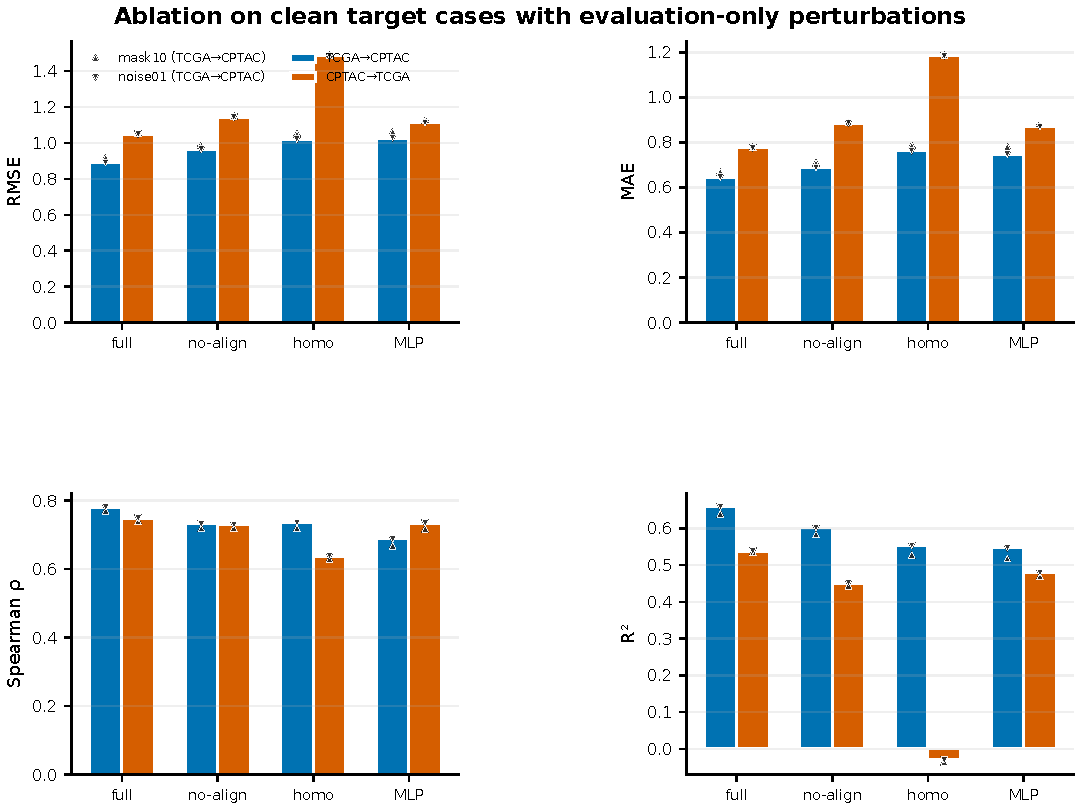
\includegraphics[width=\linewidth]{../results/figures/figure3_ablation.pdf}
\caption{Confirmatory ablation across both external directions. Bars show clean held-out performance for the full heteroscedastic/domain variant, no-domain heteroscedastic, homoscedastic/domain, and mean-only neural controls after the same source development, all-source refit, target adaptation, and held-out evaluation protocol. Triangles mark the corresponding scores after evaluation-only masking of 10\% of standardized genes or addition of Gaussian noise using the same held-out cases and fixed target adaptation batch; colors identify the two cohort directions.}
\label{fig:ablation}
\end{figure}

In CPTAC$\rightarrow$TCGA, the full model had mean RMSE $1.049\pm0.034$ and $R^2=0.538\pm0.036$, compared with RMSE $1.143\pm0.040$ and $R^2=0.451\pm0.034$ after removing domain alignment. The homoscedastic domain model degraded to RMSE $1.484\pm0.637$ and $R^2=-0.030\pm0.868$, with one seed producing a catastrophic error. In TCGA$\rightarrow$CPTAC, the full model had RMSE $0.891\pm0.019$ and $R^2=0.660\pm0.023$, compared with RMSE $0.963\pm0.037$ and $R^2=0.603\pm0.014$ without domain alignment. The mean-only MLP reached RMSE $1.027\pm0.039$ and $R^2=0.549\pm0.017$ in that direction and RMSE $1.113\pm0.065$ and $R^2=0.479\pm0.051$ in the reverse direction. The matched refit therefore supports both the heteroscedastic head and the domain objective, while retaining the direction-specific limitation that alignment gains are larger when CPTAC is the source.

Masking 10\% of genes increased RMSE by approximately 0.01--0.02 in the matched runs and reduced Spearman correlation by less than 0.02. Adding noise at standard deviation 0.1 produced smaller changes than seed-to-seed variation. These perturbations indicate that the model does not depend on a single exact expression vector, but they do not establish robustness to all missingness mechanisms or platform-specific normalization changes.

The ablation also clarifies why the two uncertainty mechanisms should not be conflated. Removing the variance head while retaining alignment caused the largest degradation, especially in the reverse direction, whereas removing domain alignment preserved a measurable but smaller signal. Thus, the variance head changes the regression geometry even when the point prediction head is unchanged, whereas the domain term changes the representation through a separate gradient path. The direction-specific behavior is a measured property of the assay shift, not a consequence of comparing different preprocessing routines.

\subsection{Prediction intervals expose a directional reliability limit}
The variance head produces patient-specific scale estimates. We recalibrated the scale with source validation residuals only and evaluated 50\%, 90\%, and 95\% interval coverage on external patients. Figure~\ref{fig:calibration} shows calibration bins and error by observed WMB quartile. In TCGA$\rightarrow$CPTAC, the mean per-seed 90\% coverage was $0.872\pm0.059$ and 95\% coverage was $0.917\pm0.048$. In CPTAC$\rightarrow$TCGA, coverage was $0.763\pm0.134$ at 90\% and $0.829\pm0.105$ at 95\%, indicating substantial and variable undercoverage. Tail coverage was lower than the corresponding mean in both directions. These intervals are source-calibrated diagnostics, not target-calibrated confidence statements; per-seed values and unique-patient counts are retained in the analysis tables.

\begin{figure}[t]
\centering
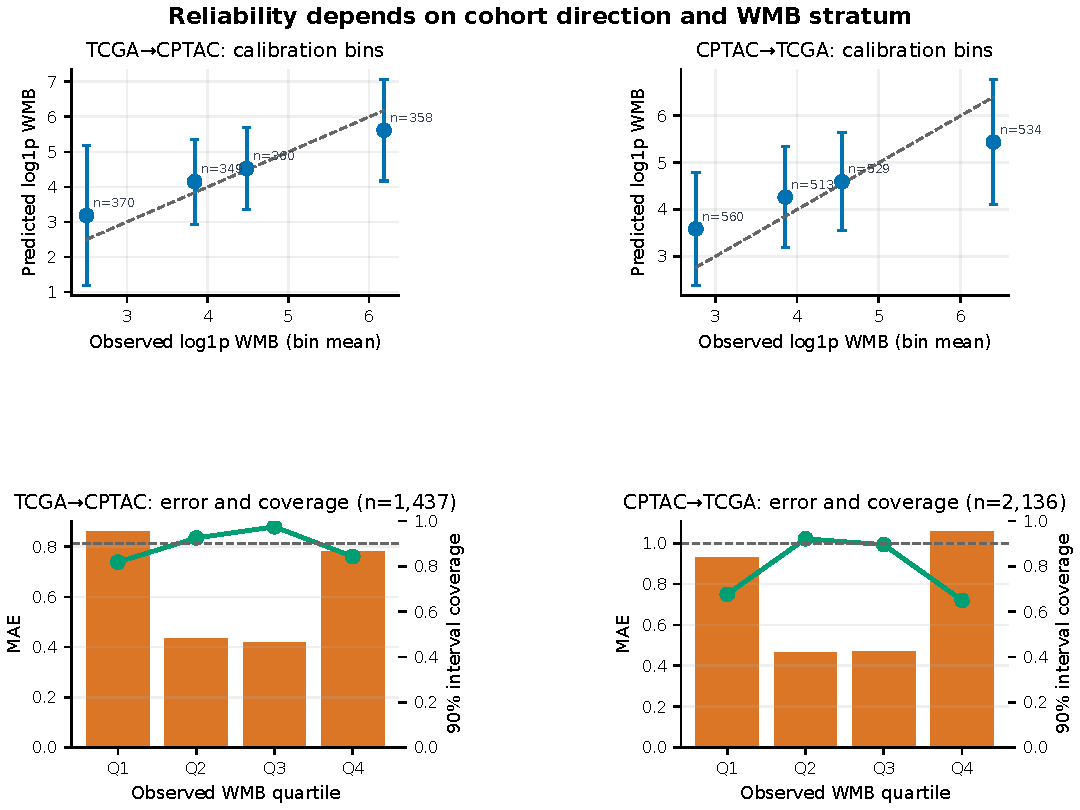
\includegraphics[width=\linewidth]{../results/figures/figure4_calibration.pdf}
\caption{External calibration and error stratification. Top panels show mean observed and predicted log1p WMB in four observed-WMB bins with the source-calibrated 90\% interval. Bottom panels show MAE as bars and empirical 90\% coverage as a line for observed-WMB quartiles. Repeated seed predictions are averaged to one value per unique held-out patient (1,437 CPTAC and 2,136 TCGA in the descriptive plots); the reverse direction under-covers both tails.}
\label{fig:calibration}
\end{figure}

The scale is informative but imperfect. Patients in the highest predicted-scale quartile had larger MAE than patients in the lowest-scale quartile in both directions, showing that uncertainty tracks some difficult examples. However, the highest WMB group can still be under-covered because residuals are asymmetric and the source and target WMB distributions differ. We therefore describe the intervals as source-calibrated rather than calibrated on the external cohort. A narrow interval is not evidence that an external case is reliable, and a source-calibrated average interval does not guarantee calibration within a lineage or WMB tail.

The calibration failure is asymmetric rather than a global variance inflation. In TCGA$\rightarrow$CPTAC, the average interval width was approximately 2.93 log1p units and 95\% coverage was 0.917 across seeds. In CPTAC$\rightarrow$TCGA, width was approximately 2.35 and 95\% coverage was 0.829 despite the larger point-error variance. This occurs because the source residual scale is not a complete description of the target residual distribution. A post-hoc target recalibration would improve these numbers but would violate the external protocol, so we report the failure and retain source-only calibration.

\subsection{Lineage errors identify where transport is weakest}
We averaged repeated seed predictions for descriptive lineage analyses; no lineage was used for model selection and repeated seed rows were not counted as additional patients. The lowest MAE occurred in KIRC (0.411 in TCGA$\rightarrow$CPTAC and 0.444 in CPTAC$\rightarrow$TCGA), while GBM was also relatively low in absolute error but had weak rank correlation. The largest errors occurred in SKCM (MAE 0.882, RMSE 1.154 for TCGA$\rightarrow$CPTAC), LAML (MAE 0.932, RMSE 1.247 for CPTAC$\rightarrow$TCGA), and UCEC (MAE 0.897, RMSE 1.214 for CPTAC$\rightarrow$TCGA). These strata have different expression programs, mutation processes, and cohort composition, so a pooled score would obscure clinically important variation. The lineage results support using the model as a prioritization tool with cohort- and lineage-specific quality checks rather than as a replacement for DNA-based measurement.

The lineage pattern is not explained by sample size alone. UCEC has the largest TCGA-to-CPTAC external count but remains among the highest-error groups, whereas GBM has fewer cases and low MAE but weak Spearman correlation. This suggests that absolute error and ranking error capture different failure modes. In low-burden lineages, a modest absolute shift can reverse ranking; in high-burden lineages, a compressed prediction range can preserve rank while producing large absolute error. We therefore retain both error families in the report and do not summarize lineage behavior with one composite score.

\subsection{Attributions are reproducible within direction but not universal across cohorts}
We computed gradient-times-input attributions for 512 held-out external patients per seed and direction using the frozen confirmatory refit models and source-derived standardized expression. The zero-centered baseline is implicit in the standardized coordinates; this is a local gradient-times-input audit rather than path-integrated attribution. The top-ranked features differed substantially between directions: the top-50 overlap was 6 genes (Jaccard 0.064), and the genome-wide rank correlation was 0.173. The highest-ranked features were reported by their stable Ensembl identifiers because gene-level interpretation is sensitive to annotation and preprocessing; they should not be interpreted as causal drivers or universal biomarkers. They are features that support a model trained under a particular assay shift.

\begin{figure}[t]
\centering
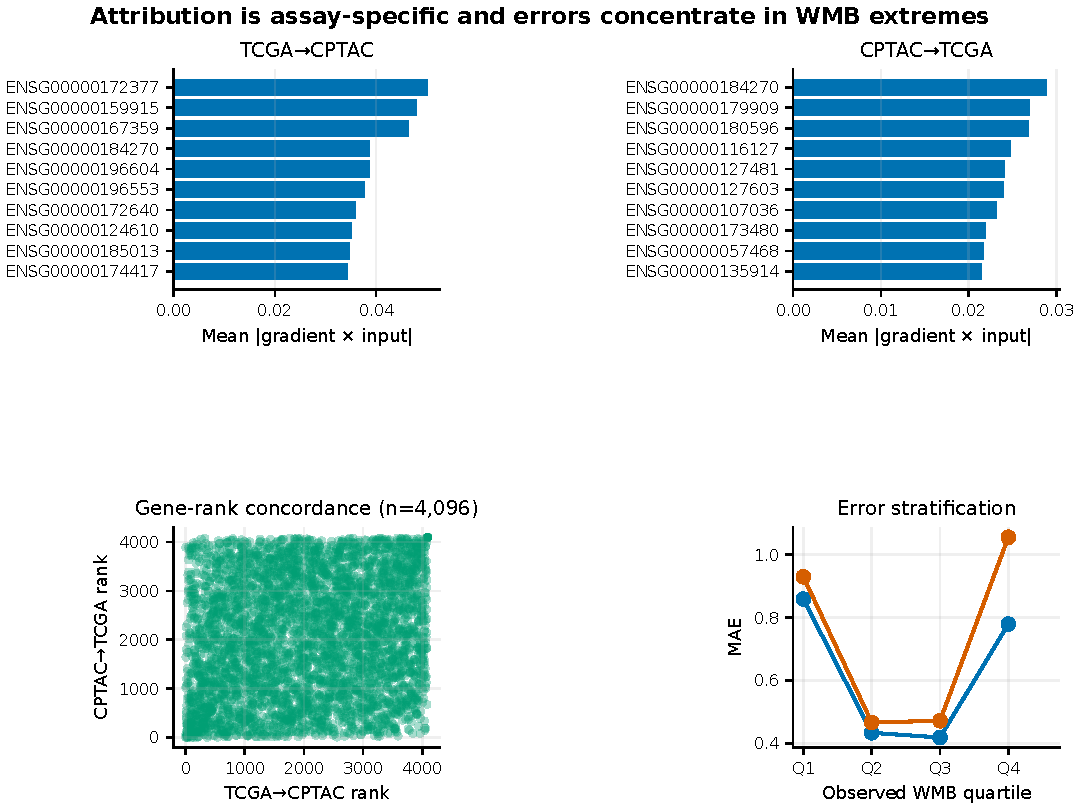
\includegraphics[width=\linewidth]{../results/figures/figure5_attribution.pdf}
\caption{Attribution and stratified error. Top panels show the ten genes with highest mean absolute gradient-times-input attribution in each direction. Bottom left compares gene ranks across directions; bottom right shows MAE by observed WMB quartile. Low overlap between attribution rankings and higher tail errors argue against interpreting individual expression genes as assay-independent WMB biomarkers.}
\label{fig:attribution}
\end{figure}

Attribution sign consistency was summarized across the three confirmatory seeds within each direction, but this consistency is conditional on the fitted representation and does not resolve confounding by lineage, purity, or technical processing. We use attributions as an audit of what the model uses, not as a post-hoc justification for the performance claim. The weak cross-direction concordance is itself a useful result because it warns that interpretation can shift when the assay direction changes even when the aggregate ranking metric remains similar.

\section{Discussion}
This study addresses a transport problem that is often hidden by random patient splits. The central result is that a single expression-based regressor improves all four reported external metrics in both directions under a source-only development and fixed refit protocol when the model explicitly represents assay shift and predictive scale. The gain over PCA-histogram boosting is approximately 0.15 log1p RMSE units when CPTAC is the source and 0.14 when TCGA is the source. The matched ablation supports both the alignment and variance mechanisms, while also showing that alignment gains are direction-dependent. These observations support a bounded interpretation: representation alignment helps under these two cohort shifts, but the result does not establish assay invariance or clinical interchangeability.

The variance head provides a second type of evidence. It distinguishes middle-range WMB cases from extreme tails where coverage falls, although neither direction reaches nominal target coverage uniformly. This is preferable to reporting a single confidence score because it makes a reliability failure visible. At the same time, source-only calibration cannot correct all target shifts. In the reverse direction, calibration slope greater than one indicates that predictions are compressed relative to external observations. A model-selection procedure that optimized only RMSE could miss this failure; a clinically oriented system should expose it.

The results complement DNA-based WMB estimation rather than replace it. The target was defined from WXS mutation calls, and the model learns a transcriptomic surrogate whose validity is bounded by that definition. Expression can reflect mutation-associated biology, but it also reflects immune composition, tissue lineage, purity, and processing. The lineage analysis and direction-specific attributions make this limitation concrete. The model performs well on aggregate metrics while remaining weak in selected strata. Such heterogeneity is expected for a biomarker that aggregates multiple mutational processes, and it argues for reporting uncertainty and lineage-specific error with every external prediction.

Several design choices strengthen the evidence. Target labels are corrected before splitting and are independent of expression. The two cohorts are never pooled for model selection. Baselines include source-mean, regularized linear models, a tree model with PCA compression, and a neural model. The candidate is compared at the individual-seed level, not only after selecting a favorable checkpoint. The corrected ablation reuses the exact training implementation and separates heteroscedasticity from domain alignment. Perturbation experiments, bootstrap comparisons, calibration bins, lineage errors, and gradient-times-input attributions answer distinct questions. Together they reduce the risk that the result is an artifact of one metric or one random seed.

The study also has clear limitations. First, TCGA and CPTAC are cohorts rather than randomized assays, and residual clinical and lineage imbalance can remain after expression normalization. Second, the WXS labels are derived from open masked files and may differ from each consortium's clinical WMB pipeline. Coordinate-and-allele deduplication avoids duplicated counting but cannot recover variants absent from an open file or correct all purity and callable-territory differences. Third, the model uses a fixed 4,096-gene panel and does not incorporate DNA, copy number, histology images, or clinical treatment. Fourth, interval calibration is source-only and under-covers target tails in one direction. Fifth, gradient-times-input attributions are model-dependent and do not establish biological causality. Finally, the present evidence covers two cohorts and eight recurrent lineages; independent prospective cohorts and platform-specific RNA normalization tests are needed before clinical use.

Future work should test whether DNA-derived covariates, explicit lineage conditioning, or conformal calibration improve tail coverage without sacrificing external point accuracy. A useful extension would predefine a third independent cohort and evaluate whether a model selected on the two existing directions preserves its advantage. Another would compare transcriptomic representations pretrained on a large, independent cancer collection with the from-scratch encoder under the same frozen external protocol. Such experiments should retain the current two-way evaluation and should be considered successful only when gains persist across all primary metrics and seeds.

\section{Methods}
\subsection{Cohort and molecular data}
The analysis uses publicly available TCGA and CPTAC-3 cases with a matched expression profile and an open masked WXS mutation file. Case identity was joined through stable GDC case identifiers. Expression values are log1p TPM values generated from GDC STAR counts and restricted to a fixed panel of 4,096 genes selected before model fitting. The panel and sample order are frozen in the processed matrix. Cohort, lineage, file identifier, mutation count, and transformed target are recorded for every retained case.

\subsection{WMB label construction}
\sloppy
For every case, all WXS MAF records with one of the following exact ``Variant\_Classification'' values were retained:
\begin{quote}\footnotesize\raggedright\texttt{Frame\_Shift\_Del}, \texttt{Frame\_Shift\_Ins}, \texttt{In\_Frame\_Del}, \texttt{In\_Frame\_Ins}, \texttt{Missense\_Mutation}, \texttt{Nonsense\_Mutation}, \texttt{Nonstop\_Mutation}, \texttt{Splice\_Site}, \texttt{Translation\_Start\_Site}, \texttt{Multi\_Hit}.\end{quote}
\noindent Synonymous, intronic, intergenic, and records lacking a valid genomic coordinate or allele were excluded. A variant key consisted of chromosome, start, end, reference allele, and alternate allele. Duplicate keys were counted once, including duplicates observed in multiple files for a case. The files are masked WXS calls and were used with their supplied GDC genome-build coordinates; no additional left-alignment or caller-specific quality filter was applied. The target is the natural logarithm of one plus this unique count. It is therefore a WXS mutation burden (WMB), not mutations per megabase: callable territory, purity, depth, and capture differences are not normalized. We audited label construction by comparing counts before and after deduplication and by verifying that no expression column was read by the label builder. Cases without an open WXS file were excluded before any split.
\fussy

\subsection{External split and preprocessing}
For each direction, source cases were split 80:20 with \texttt{train\_test\_split} and a fixed random state of 11, 23, or 47 during source-only development. The frozen architecture, optimizer, epoch budget, and calibration rule were then refit on all source patients. The target cohort was split 50:50 with random state seed+9000 into an unlabeled adaptation subset and a disjoint external evaluation subset. Only adaptation expression is passed to the domain discriminator; evaluation expression and all target labels are absent from fitting and are consumed only for final scoring. Missing expression values were replaced with zero after source-derived standardization. The source-derived mean and standard deviation used for the refit are frozen from the development protocol and are applied to both target subsets; features with source standard deviation below $10^{-5}$ were assigned unit scale. No target statistic was used for normalization, and target labels were not consumed during fitting.

\subsection{Baselines}
The source-mean predictor uses the mean transformed target in all source patients after source-only development. Ridge and elastic-net regressions use standardized expression with regularization selected within source validation and are refit on all source labels. The PCA-histogram gradient boosting baseline projects expression onto principal components fitted using source-derived preprocessing and fits histogram gradient boosting to all source targets after its source-only choice. A neural MLP uses the same encoder dimensions as the candidate but a single mean head and a squared-error loss; it does not consume target adaptation expression. These baselines cover constant, linear, tree, and neural families. Every confirmatory method therefore receives the same source-label set. The assay-aware candidate and homoscedastic-domain control use the unlabeled adaptation batch for alignment, whereas PCA-HGB, ridge, elastic-net, and the mean-only/heteroscedastic no-domain controls are inductive; target labels are never used for tuning.

\subsection{Assay-aware heteroscedastic model}
The encoder maps a standardized expression vector $x\in\mathbb{R}^{4096}$ to a 128-dimensional representation $h$. Layer normalization and GELU activations stabilize the projection, and dropout is applied in the first hidden layer. The mean and log-variance heads produce $\mu(h)$ and $\ell(h)$. The Gaussian negative log-likelihood is evaluated only on labeled source patients. The discriminator maps $h$ to a cohort logit. Source representations have domain target zero and unlabeled target representations have domain target one. A gradient reversal operator leaves the forward representation unchanged but multiplies its backward gradient by a negative coefficient. The coefficient follows $0.35[2/(1+\exp(-8t/T))-1]$ over epoch $t$ and total epochs $T$.

Training uses AdamW with learning rate $2\times10^{-3}$, weight decay $2\times10^{-4}$, mini-batches of 128, gradient norm clipping at 5, and a fixed epoch budget selected during source-only development. The source-development runs fix the architecture, optimizer, and 50-epoch schedule; no external checkpoint is selected. The final point predictor is then refit on all source patients. The multiplicative residual calibration factor is carried forward from independent source-validation predictions from the development fit; it is never estimated from predictions of the all-source refit. For external prediction, the standard deviation is $\sigma=\exp(\ell/2)$ after clipping $\ell$ to $[-6,4]$, multiplied by this frozen source-validation factor. The 90\% interval is $\mu\pm1.64485\sigma$.

\subsection{Ablation and robustness}
The matched ablation changes one mechanism at a time while retaining the same data split, standardization, optimizer, fixed 50-epoch schedule, and seed schedule. The no-domain model removes the discriminator. The zero-domain-coefficient model keeps the discriminator but sets its supervised contribution to zero. The homoscedastic model replaces the sample-specific log variance with a scalar. A mean-only MLP removes both variance and domain adaptation. Robustness is evaluated by masking 10\% of standardized expression entries using a seed-specific random mask and by adding independent Gaussian noise with standard deviation 0.1. These perturbations are applied only to the external expression matrix at evaluation time.

\subsection{Metrics and uncertainty analysis}
Primary metrics are RMSE, MAE, Spearman correlation, and coefficient of determination $R^2$. RMSE and MAE are in log1p mutation-count units. Spearman correlation is computed on external predictions and is not used for model selection. We use a continuous log1p count because it preserves information across the burden range and permits tail error and interval analyses without choosing an external threshold. Calibration slope and intercept are descriptive ordinary least-squares estimates of observed target on predicted mean. Coverage is the proportion of patients satisfying $|y-\mu|\le z\sigma$ for $z\in\{0.67449,1.64485,1.95996\}$.

The confirmatory specification was fixed during source-only development. Each direction and seed uses source-derived standardization, a fixed 50-epoch budget, and an all-source refit; conventional baselines receive the same source-label set. The target cohort is split before fitting into an unlabeled adaptation half and a disjoint evaluation half. Target labels are consumed only for the final external score, and no target metric selects the architecture, schedule, calibration, or checkpoint. Patient-level bootstrap resamples each fixed external evaluation set 2,000 times for paired candidate-minus-CORAL differences; the resulting intervals are descriptive patient-resampling uncertainty and do not represent cohort-level transportability. Between-seed variation is reported separately as mean $\pm$ standard deviation. Lineage summaries collapse repeated seeds to unique patients, while error-stratum analyses use direction-specific quartiles of observed WMB or predicted scale.

\subsection{Attribution}
Gradient-times-input attributions are computed on frozen confirmatory refit models using source-derived standardized expression. For each direction and seed, 512 held-out evaluation patients are sampled with a fixed seed; the output gradient is multiplied elementwise by the observed standardized input. Absolute attribution is averaged across patients and seeds, and signed attribution and sign consistency are retained. We report top-feature lists, top-50 overlap, Jaccard similarity, and Spearman correlation of genome-wide ranks. Attribution is used to audit model reliance and is not interpreted as a causal estimate.

\section*{Ethics statement}
This computational analysis used de-identified, publicly available TCGA and CPTAC molecular records accessed through the Genomic Data Commons. No participants were recruited, contacted, or re-identified for this study; source-consortium access and data-use terms apply.

\section*{Competing interests}
The authors declare no competing interests.

\section*{Author contributions}
Author names and contribution assignments will be completed in the submission metadata.

\section{Data and code availability}
The study uses publicly available TCGA and CPTAC molecular data accessed through the NCI Genomic Data Commons (TCGA project: \url{https://portal.gdc.cancer.gov/projects/TCGA}; CPTAC-3 project: \url{https://portal.gdc.cancer.gov/projects/CPTAC-3}; GDC documentation: \url{https://docs.gdc.cancer.gov/}). Queries and file manifests were frozen on 2026-10-05. Code, derived labels, split identifiers, prediction tables, figure sources, checksums, and manuscript source are archived at \url{https://github.com/jinluo12345/tcga-cptac-wmb-transport}; raw controlled-access files are not redistributed. Model weights can be regenerated from the fixed seeds and source-only preprocessing. No DOI is assigned.

\section{Reporting summary}
The sample counts, data exclusions, preprocessing rules, seeds, metrics, uncertainty definitions, ablation variants, corruption tests, lineage strata, attribution baseline, and bootstrap procedure are specified above. No human intervention was used to choose external checkpoints or favorable lineages. The source-only development specification was fixed before final external scoring.

\bibliographystyle{unsrtnat}
\bibliography{references}
\end{document}
